\chapter{Nonlinear Derivatives and Embedded Optionality}
\label{chap:Nonlinear_Derivatives_and_Embedded_Optionality}

\begin{openingcase}{Paying for Protection Without Giving Up the Upside}

An exporter expects to receive USD~10 million in three months. The firm is concerned that the dollar may weaken before the payment arrives, reducing the renminbi value of the receivable. A forward contract can lock in an exchange rate, but it also removes the benefit of a stronger dollar.

The treasurer considers a put option instead. It can protect the receivable if the dollar weakens while preserving the gain from a stronger dollar. The difficulty is that the firm must pay for this flexibility in advance, even if the protection is never needed.

\end{openingcase}


\begin{tcolorbox}[
  enhanced,
  colback=FinanceBlue!6,
  colframe=FinanceBlue,
  boxrule=0.6pt,
  sharp corners,
  left=8pt,
  right=8pt,
  top=7pt,
  bottom=7pt,
  before skip=1em,
  after skip=1.6em,
  title=\textbf{Core Questions},
  coltitle=white,
  colbacktitle=FinanceBlue,
  fonttitle=\bfseries,
  attach boxed title to top left={xshift=6pt,yshift=-2mm},
  boxed title style={
    boxrule=0pt,
    sharp corners,
    left=5pt,
    right=5pt,
    top=2pt,
    bottom=2pt
  }
]
\begin{enumerate}[
  leftmargin=*,
  label=\textcolor{FinanceBlue}{\textbf{\arabic*.}},
  itemsep=0.55em,
  topsep=0.2em
]


\item How do option rights create asymmetric payoffs, in
contrast to the linear payoff structures of forward,
futures, and swap contracts?

\item What determines option value, and how do replication, risk-neutral valuation, and option sensitivities help explain both standalone options and optionality embedded in financial contracts?

\end{enumerate}
\end{tcolorbox}


\section{Option Logic and Asymmetric Payoffs}

An option gives its holder a contractual right without imposing the same obligation to act. The writer accepts the corresponding contingent obligation. This asymmetry creates nonlinear payoffs, since exercise depends on whether the realized state makes the contractual right valuable.

Option value before maturity depends on the underlying price, strike price, time to maturity, volatility, financing conditions, and contract design. Similar optionality can also be embedded in bonds, mortgages, and other financial claims.

\subsection{Calls, Puts, and Exercise Rights}

A call option gives its holder the right to buy the underlying asset at strike price \(K\), while a put option gives the right to sell at \(K\). A European option can be exercised only at maturity \(T\), whereas an American option may be exercised at any time up to maturity.

For a European option, the payoff at maturity is

\begin{equation}
C_T=\max\{S_T-K,0\},
\label{eq:ch18-call-payoff}
\end{equation}
and
\begin{equation}
P_T=\max\{K-S_T,0\}.
\label{eq:ch18-put-payoff}
\end{equation}

The call is exercised at maturity when \(S_T>K\), while the put option is exercised when \(S_T<K\). Otherwise, the option expires without exercise. The writer bears the corresponding payoff obligation.

For an American option, exercise may occur at an earlier date \(\tau \le T\). The same payoff logic applies using the underlying price \(S_\tau\) at the exercise date.

The premium paid at inception is separate from the
exercise payoff. Let $\Pi_T$ denote the option buyer's
net profit at expiration, calculated as the exercise
payoff minus the initial premium. For a call purchased
for $c_0$,

\begin{equation}
\Pi_T^{\mathrm{call}}
=
\max\{S_T-K,0\}-c_0,
\label{eq:ch18-call-profit}
\end{equation}

while a put option purchased for \(p_0\) has

\begin{equation}
\Pi_T^{\mathrm{put}}
=\max\{K-S_T,0\}-p_0.
\label{eq:ch18-put-profit}
\end{equation}

A positive exercise payoff may still be insufficient to recover the premium.

\begin{example}{A Call Right and the Premium}{call-right-premium}

A six-month call option has a strike price of RMB~50 and costs RMB~4. If the stock price at maturity is RMB~62, the payoff is RMB~12 and the profit is RMB~8, ignoring financing of the premium. If the stock price is RMB~48, the option expires without exercise and the holder loses the RMB~4 premium.

\end{example}

For an American option, the ability to exercise early expands the holder's choice set, but early exercise need not be optimal. Remaining time value, cash distributions, interest rates, and contract terms can make continued holding more valuable than immediate exercise.




\subsection{Asymmetric Hedging and Payoff Reshaping}

Options can modify an existing exposure by changing payoffs in selected states. Consider an investor who owns one share and buys a put option with strike \(K\). Excluding the option premium, the maturity payoff is

\begin{equation}
V_T^{\mathrm{protective\ put}}
=S_T+\max\{K-S_T,0\}=
\max\{S_T,K\}.
\label{eq:ch18-protective-put}
\end{equation}

The put option places a floor at \(K\) while preserving gains when the stock price rises above the strike. The premium paid for this protection reduces the investor's net return across states.

A similar mechanism can limit the cost of a future purchase. Suppose a firm plans to buy one unit of a commodity at maturity and holds a call option with strike \(K\). Excluding the premium, the effective purchase cost is

\begin{equation}
S_T-\max\{S_T-K,0\}
=\min\{S_T,K\}.
\label{eq:ch18-call-hedged-purchase}
\end{equation}

The call option places a ceiling on the effective purchase price while preserving the benefit of a decline below \(K\). A forward hedge, by contrast, tends to fix the effective purchase price when the contract and underlying exposure are closely matched.

\begin{table}[H]
\centering
\caption{Linear and option-based hedging of a future purchase}
\label{tab:ch18-forward-option-hedge}
\begin{tabularx}{\textwidth}{@{}p{3.2cm}YY@{}}
\toprule
\textbf{Position} &
\textbf{Adverse price increase} &
\textbf{Favorable price decline} \\
\midrule
Long forward &
Higher purchase cost is largely offset when the hedge closely matches the exposure &
Forward losses offset much of the benefit from the lower spot price \\
Long call &
Protection increases once the price rises above the strike &
The option can expire unused, allowing the lower spot price to be retained \\
\bottomrule
\end{tabularx}
\end{table}

Options can also exchange exposure in one set of states for a premium received at inception. An investor who owns one share and sells a call option with strike \(K\) has, excluding the premium received,

\begin{equation}
V_T^{\mathrm{covered\ call}}
=S_T-\max\{S_T-K,0\}
=\min\{S_T,K\}.
\label{eq:ch18-covered-call}
\end{equation}

The premium is received at inception, while gains above \(K\) are surrendered. The protective put, long call hedge, and covered call illustrate the same mechanism: option positions redistribute exposure across states rather than changing all states in the same proportion.



\subsection[Optionality as Economic Flexibility under Uncertainty]{Optionality as Economic Flexibility under Uncertainty}

Optionality preserves the ability to make a decision after uncertainty has been partly resolved. Unlike a contract that fixes future action in advance, an option allows the holder to respond to the state that later emerges, subject to the contract's exercise terms.

This flexibility is valuable when future conditions are uncertain and decisions are costly to reverse. A call option can limit the purchase price of an input while preserving the benefit of a price decline. A put option can establish a floor on an asset position while retaining gains if the asset price rises. The option does not remove uncertainty; it changes how the holder participates in different future states.

The same principle appears in financial claims with embedded options. A convertible bond gives the investor the right to exchange debt for equity, a callable bond gives the issuer the right to redeem the bond before maturity, and a prepayable mortgage allows the borrower to repay early under specified terms. In each case, optionality assigns future decision rights and changes the distribution of cash flows across states.

\subsection[Options for Hedging, Speculation, and Premium Income]{Options for Hedging, Speculation, and Premium Income}

The economic role of an option depends on the exposure with which it is combined. Options may be used to modify an existing risk, create a new market exposure, or receive premium income in exchange for accepting a contingent obligation.

In hedging, the option is combined with an existing or expected exposure. A call option can limit the cost of a future purchase, while a put option can protect the value of a future sale or an asset position. The option changes losses in selected adverse states without necessarily removing favorable exposure.

In speculation, the option itself creates exposure to movements in the underlying variable. A call option provides exposure to price increases, while a put option provides exposure to price declines. Since the premium may be small relative to the underlying exposure, changes in option value can produce large percentage gains or losses relative to the initial investment.

In premium-income strategies, the investor receives the option premium and accepts the associated contingent obligation. A covered call option gives up part of the potential gain above the strike, while a cash-secured put option creates the possibility of purchasing the underlying asset if exercise occurs.

These uses differ in purpose, but each reflects the same contractual mechanism: option rights and obligations redistribute cash flows across future states.

\section{Option Valuation and Economic Intuition}

Option value before expiration can differ from immediate exercise value. An out-of-the-money option may still have positive value, while an in-the-money option may be worth more than the payoff from immediate exercise. Time remaining preserves the possibility that future price movements will make the exercise right more valuable.

\subsection{Determinants of Option Value}

The value of a standard option depends on the underlying price \(S_t\), strike price \(K\), time to maturity, volatility, interest rates, and relevant cash distributions or carrying benefits.

Moneyness describes the relation between the underlying
price and the strike price. A call option is in the money
when $S_t>K$ and out of the money when $S_t<K$; for a put
option, the conditions are reversed. An option is at the
money when $S_t=K$ or approximately at the money when
the two prices are close.

The intrinsic values of call and put options are

\begin{equation}
I_t^{C}=\max\{S_t-K,0\},
\qquad
I_t^{P}=\max\{K-S_t,0\}.
\label{eq:ch18-option-intrinsic}
\end{equation}

These expressions show that an in-the-money option has
positive intrinsic value, whereas an out-of-the-money or
at-the-money option has zero intrinsic value.

The difference between an option's market value and its
intrinsic value is commonly described as time value. It
reflects, among other factors, the possibility that future
price movements may make the exercise right more valuable.
For some European options, however, this difference need
not be positive under all market conditions.

Volatility has a particularly important effect on option value. Greater dispersion in future prices expands the range of favorable exercise states, while the holder is not required to exercise in unfavorable states. Under standard pricing conditions, higher volatility tends to increase the value of both calls and puts.

Time to maturity affects value through the opportunity for future states to evolve. A longer maturity may increase the value of flexibility, although the effect can depend on interest rates, cash distributions, carrying costs, and exercise features. Interest rates and dividends also alter the relative value of receiving or paying cash at different dates.

\begin{table}[H]
\centering
\caption{Typical comparative effects on European stock-option values}
\label{tab:ch18-option-value-determinants}
\begin{tabular}{@{}lcc@{}}
\toprule
\textbf{Increase in input} & \textbf{Call value} & \textbf{Put value} \\
\midrule
Underlying price \(S_t\) & Higher & Lower \\
Strike price \(K\) & Lower & Higher \\
Volatility \(\sigma\) & Higher & Higher \\
Time to maturity & Usually higher & May be higher or lower \\
Risk-free rate \(r\) & Higher & Lower \\
Dividend yield \(q\) & Lower & Higher \\
\bottomrule
\end{tabular}
\end{table}

These directions describe standard European stock options under familiar pricing conditions. The effect of maturity is less uniform than the effects of the underlying price, strike, or volatility.

\subsection[Binomial Valuation: Replication in Discrete States]{Binomial Valuation: Replication in Discrete States}

The binomial model values an option by reproducing its payoffs across discrete future states. Suppose a stock with current price \(S_0\) will move to either \(S_u\) or \(S_d\) after one period. A call option with strike \(K\) has payoffs

\begin{equation*}
C_u=\max\{S_u-K,0\},
\qquad
C_d=\max\{S_d-K,0\}.
\label{eq:ch18-binomial-call-payoffs}
\end{equation*}

\begin{figure}[H]
\centering
\begin{tikzpicture}[
 =stealth,
 node distance=2.4cm,
 every node/.style={font=\small}
 ]

\node (s0) [align=center] {
\(S_0\),
\(C_0\)
};

\node (su) [right=4.5cm of s0, yshift=1.5cm, align=center] {
\(S_u\),
\(C_u=\max\{S_u-K,0\}\)
};

\node (sd) [right=4.5cm of s0, yshift=-1.5cm, align=center] {
\(S_d\),
\(C_d=\max\{S_d-K,0\}\)
};

\draw[->] (s0) -- node[above, sloped] {Up state} (su);
\draw[->] (s0) -- node[below, sloped] {Down state} (sd);

\end{tikzpicture}

\caption{One-period binomial structure for a call option}
\label{fig:ch18-one-period-binomial}
\end{figure}

A portfolio containing \(\Delta\) shares and a risk-free position \(B\) replicates these payoffs when

\begin{align*}
\Delta S_u+B(1+r)&=C_u,\\
\Delta S_d+B(1+r)&=C_d.
\end{align*}

Solving the two equations gives

\begin{equation}
\Delta
=\frac{C_u-C_d}{S_u-S_d},
\label{eq:ch18-binomial-delta}
\end{equation}

and

\begin{equation}
B
=\frac{C_d-\Delta S_d}{1+r}.
\label{eq:ch18-binomial-bond}
\end{equation}

Under no-arbitrage conditions, the option value equals the current cost of the replicating portfolio:

\begin{equation}
C_0=\Delta S_0+B.
\label{eq:ch18-binomial-value}
\end{equation}

The valuation follows from reproducing the option's state-contingent payoffs rather than from forecasting which state will occur.

In the one-period binomial tree shown in
Figure~\ref{fig:ch18-one-period-binomial}, the initial stock
price $S_0$ can move to either $S_{u}=uS_0$ in the up state
or $S_{d}=dS_0$ in the down state. Let $q$ denote the
risk-neutral probability assigned to the up state,
so that $1-q$ is the probability assigned to the
down state.

Under risk-neutral valuation, the expected future
stock price, discounted at the risk-free rate, must
equal its current price. Thus,

\begin{equation*}
S_0=\frac{quS_0+(1-q)dS_0}{1+r}.
\end{equation*}

Rearranging gives

\begin{equation*}
1+r=qu+(1-q)d.
\end{equation*}

Solving for $q$ gives the risk-neutral probability

\begin{equation}
q=\frac{(1+r)-d}{u-d}.
\label{eq:ch18-binomial-risk-neutral-probability}
\end{equation}

\begin{example}{One-Period Call Option Valuation}{one-period-call-ch18}

A stock sells for RMB~100 and will be either RMB~120 or RMB~80 in one year. The risk-free rate is 5\%, and a call has a strike price of RMB~100. Its payoffs are RMB~20 in the up state and zero in the down state. Hence,

$$
\Delta=\frac{20}{120-80}=0.5,
$$

and

$$
B=\frac{0-0.5\times 80}{1.05}=-38.095.
$$

The call option value is

$$
C_0=0.5\times 100-38.095=11.905.
$$

\end{example}

The same logic extends to successive periods. In a two-period tree, terminal payoffs are determined first and earlier node values are obtained by backward induction.

\begin{figure}[H]
\centering
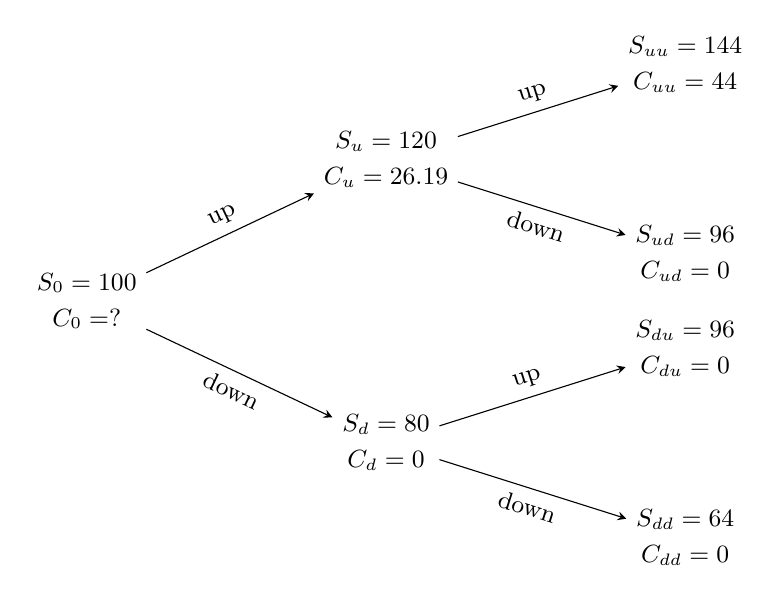
\begin{tikzpicture}[
    >=stealth,
    every node/.style={font=\small},
    level 1/.style={sibling distance=42mm},
    level 2/.style={sibling distance=24mm}
]

\node (S0) at (0,0) [align=center] {$S_0=100$\\[2pt] $C_0=?$};

\node (Su) at (3.8,1.8) [align=center] {$S_u=120$\\[2pt] $C_u=26.19$};
\node (Sd) at (3.8,-1.8) [align=center] {$S_d=80$\\[2pt] $C_d=0$};

\node (Suu) at (7.6,3.0) [align=center] {$S_{uu}=144$\\[2pt] $C_{uu}=44$};
\node (Sud) at (7.6,0.6) [align=center] {$S_{ud}=96$\\[2pt] $C_{ud}=0$};
\node (Sdu) at (7.6,-0.6) [align=center] {$S_{du}=96$\\[2pt] $C_{du}=0$};
\node (Sdd) at (7.6,-3.0) [align=center] {$S_{dd}=64$\\[2pt] $C_{dd}=0$};

\draw[->] (S0) -- node[above,sloped] {up} (Su);
\draw[->] (S0) -- node[below,sloped] {down} (Sd);

\draw[->] (Su) -- node[above,sloped] {up} (Suu);
\draw[->] (Su) -- node[below,sloped] {down} (Sud);

\draw[->] (Sd) -- node[above,sloped] {up} (Sdu);
\draw[->] (Sd) -- node[below,sloped] {down} (Sdd);

\end{tikzpicture}
\caption{Two-period binomial tree for a European call}
\label{fig:ch18-two-period-binomial}
\end{figure}




For a two-period European call, backward induction gives

\begin{equation}
C_u=
\frac{qC_{uu}+(1-q)C_{ud}}{1+r},
\qquad
C_d=
\frac{qC_{du}+(1-q)C_{dd}}{1+r},
\label{eq:ch18-binomial-one-period-backward}
\end{equation}
and

\begin{equation}
C_0=
\frac{qC_u+(1-q)C_d}{1+r}.
\label{eq:ch18-binomial-two-period-backward}
\end{equation}

\begin{example}{Two-Period Call Valuation}{two-period-call-valuation}

Suppose \(S_0=100\), with \(u=1.2\), \(d=0.8\), and a risk-free rate of 5\% per period. A European call option has strike price \(K=100\) and maturity of two periods.

At maturity, the stock prices are \(144\), \(96\), and \(64\), giving call option payoffs of \(44\), \(0\), and \(0\). The risk-neutral probability is

$$
q=\frac{1.05-0.8}{1.2-0.8}=0.625.
$$

At the first-period nodes,

$$
C_u=
\frac{0.625\times 44}{1.05}
=26.19,
\qquad
C_d=0.
$$

Moving back one more period gives

$$
C_0=
\frac{0.625\times 26.19}{1.05}
=15.59.
$$

Thus the multi-period value is obtained by working backward from terminal option payoffs through the tree.

\end{example}

The procedure extends to larger trees. For an option that can be exercised before maturity, the value at each exercise date is obtained by comparing the payoff from immediate exercise with the value of keeping the option alive.

The binomial framework makes replication transparent in discrete states. The same pricing principle can be extended to settings in which the underlying price evolves continuously.


\subsection[Black--Scholes--Merton: Risk-Neutral Pricing Intuition]{Black--Scholes--Merton: Risk-Neutral Pricing Intuition}

In continuous time, the Black--Scholes--Merton framework expresses the same no-arbitrage logic through dynamic replication. For a European call option on a non-dividend-paying stock,

\begin{equation}
C_0
=S_0N(d_1)-Ke^{-rT}N(d_2),
\label{eq:ch18-bsm-call}
\end{equation}
where

\begin{equation}
d_1
=\frac{\ln(S_0/K)+(r+\tfrac{1}{2}\sigma^2)T}{\sigma\sqrt{T}},
\qquad
d_2=d_1-\sigma\sqrt{T},
\label{eq:ch18-bsm-d1d2}
\end{equation}
and \(N(\cdot)\) is the standard normal cumulative distribution function. The corresponding European put option value is

\begin{equation}
P_0
=Ke^{-rT}N(-d_2)-S_0N(-d_1).
\label{eq:ch18-bsm-put}
\end{equation}

The pricing mechanism rests on a dynamically adjusted position in the stock and risk-free financing. As the stock price changes, the hedge is rebalanced to reproduce the option's local exposure. Under the model assumptions, no-arbitrage links the option value to the cost of this replicating strategy.

The same result can be represented through risk-neutral valuation. For pricing purposes, the stock's expected return is replaced by the risk-free rate, and the option value is obtained from the discounted expected payoff under the risk-neutral measure. This representation is consistent with replication and does not require the risk-neutral distribution to describe actual future outcomes.

The benchmark model assumes frictionless trading, continuous rebalancing, a continuous stock-price process with constant volatility, and a constant risk-free rate in its basic form. Actual markets may involve transaction costs, discrete trading, price jumps, liquidity constraints, and changing volatility, so the model is best viewed as a benchmark for valuation.

Observed option prices can also be expressed through implied volatility, defined as the value of \(\sigma\) that makes the model price equal to the market price. Once an option value is expressed as a function of its underlying inputs, the same framework can also be used to measure how that value responds to changes in those inputs.


\begin{tcolorbox}[
enhanced,
breakable,
colback=white,
colframe=FinanceBlue,
boxrule=0.7pt,
sharp corners,
borderline west={2.2pt}{0pt}{FinanceBlue},
title=\textbf{Financial Perspective: A Pricing Model Is Not a Forecast},
coltitle=white,
colbacktitle=FinanceBlue,
fonttitle=\bfseries,
before skip=1.2em,
after skip=1.2em
]

Risk-neutral pricing uses traded prices and no-arbitrage conditions to value contingent claims. The resulting risk-neutral distribution need not coincide with investors' beliefs about actual future outcomes.

\end{tcolorbox}

\subsection{Put--Call Parity and No-Arbitrage Consistency}

European call and put options written on the same underlying
asset, with the same strike price and expiration date, are
linked by a no-arbitrage relationship known as put--call
parity. The relationship follows from the equivalence of
two portfolios that generate identical payoffs at maturity.

Consider two portfolios. Portfolio A consists of a European
call option and a risk-free zero-coupon bond with face value
$K$. Portfolio B consists of a European put option and one
unit of the underlying asset. Their values at maturity are

\begin{equation*}
\begin{aligned}
W_A(T)&=\max\{S_T-K,0\}+K,\\
W_B(T)&=\max\{K-S_T,0\}+S_T.
\end{aligned}
\end{equation*}

For either $S_T\geq K$ or $S_T<K$, the two portfolios produce
the same terminal payoff:

\begin{equation*}
W_A(T)=W_B(T)=\max\{S_T,K\}.
\end{equation*}

Under no-arbitrage conditions, portfolios with identical
future payoffs must have the same current value. Let $C_0$
and $P_0$ denote the current prices of the call and put
options, respectively, and let $D(0,T)$ denote the
risk-free discount factor to the expiration date. Put--call
parity is therefore

\begin{equation}
C_0+KD(0,T)=P_0+S_0.
\label{eq:ch18-put-call-parity}
\end{equation}

Equivalently,

\begin{equation}
C_0-P_0=S_0-KD(0,T).
\end{equation}

The relationship shows that the difference between call
and put prices is determined by the underlying asset price
and the present value of the strike price. If the two sides
of equation~\eqref{eq:ch18-put-call-parity} differ, an
investor may construct offsetting positions to exploit
the pricing discrepancy.

Put--call parity provides a consistency condition for
European option prices rather than a separate pricing
model. It also illustrates how options, the underlying
asset, and risk-free borrowing or lending can be combined
to construct equivalent financial positions.

\subsection{Option Sensitivities and Dynamic Hedging}

The local responses of option value to changes in market inputs are summarized by the Greeks. Delta measures sensitivity to the underlying price,

\begin{equation}
\Delta=\frac{\partial V}{\partial S},
\label{eq:ch18-delta}
\end{equation}
while gamma measures how delta changes as the underlying price changes,

\begin{equation}
\Gamma=\frac{\partial^2 V}{\partial S^2}.
\label{eq:ch18-gamma}
\end{equation}


For a small change in the underlying asset price, the
change in option value can be approximated by

\begin{equation}
\Delta V
\approx
\frac{\partial V}{\partial S}\times\Delta S
+
\frac{1}{2}\frac{\partial^2 V}{\partial S^2}\times(\Delta S)^2.
\label{eq:ch18-delta-gamma}
\end{equation}

Delta captures the local slope of the option-value function,
while gamma captures its curvature. Standard long calls and
puts typically have positive gamma, so their deltas change
as the underlying price moves. Other Greeks describe
sensitivity to additional pricing inputs. The main option
Greeks and their corresponding sensitivities are summarized
in Table~\ref{tab:ch18-option-greeks}.

\begin{table}[H]
\centering
\caption{Selected option sensitivities}
\label{tab:ch18-option-greeks}
\begin{tabularx}{\textwidth}{@{}p{2.0cm}p{3.0cm}Y@{}}
\toprule
\textbf{Greek} & \textbf{Definition} & \textbf{Interpretation} \\
\midrule
Delta & \(\partial V/\partial S\) & Sensitivity to the underlying price \\
Gamma & \(\partial^2V/\partial S^2\) & Change in delta as the underlying price changes \\
Vega & \(\partial V/\partial \sigma\) & Sensitivity to volatility \\
Theta & \(-\partial V/\partial \tau\) & Sensitivity to the passage of time, where \(\tau\) is time to maturity \\
Rho & \(\partial V/\partial r\) & Sensitivity to the interest rate \\
\bottomrule
\end{tabularx}
\end{table}

These sensitivities provide the basis for dynamic hedging. A dealer who is short calls may buy the underlying asset to offset the position's current delta. As the underlying price changes, the option's delta also changes, so the hedge may need to be rebalanced.

Delta hedging is local rather than permanent. Discrete trading, price jumps, transaction costs, liquidity constraints, changing volatility, and model error can leave residual exposure. Greeks describe how option value responds to market changes, but they do not imply that all risk can be removed.

The need for rebalancing follows from the nonlinear structure of option value. A linear derivative has a relatively stable sensitivity to the underlying, whereas an option's sensitivity changes with market conditions.



\section{Embedded Optionality in Financial Claims}

The same option logic can appear inside securities that are not traded as standalone options. Bonds, mortgages, and structured securities may contain contractual rights that alter the timing, amount, or allocation of future cash flows when specified conditions are met.

\subsection{Convertible Bonds: Equity Options in Debt Contracts}

A convertible bond combines a debt claim with the investor's right to convert the bond into equity under specified terms. The debt component provides contractual payments, while the conversion right links part of the bond's value to the issuer's share price.

If a bond with face value \(F\) can be converted into \(m\) shares, its conversion value at time \(t\) is

\begin{equation}
CV_t=mS_t,
\label{eq:ch18-conversion-value}
\end{equation}
where \(S_t\) is the share price. Under a fixed conversion ratio, the corresponding conversion price is

\begin{equation}
K_c=\frac{F}{m}.
\label{eq:ch18-conversion-price}
\end{equation}

As the share price rises, the conversion value increases. Conversion becomes more attractive when the value of the shares received becomes large relative to the value of retaining the bond. Remaining coupon payments, redemption value, call provisions, and other contract terms can affect this comparison.

From a valuation perspective, a convertible bond combines
the value of a straight bond with the value of the
conversion option:

\begin{equation}
V_{\mathrm{convertible}}
\approx
V_{\mathrm{straight\ bond}}
+
V_{\mathrm{conversion\ option}}.
\label{eq:ch18-convertible-decomposition}
\end{equation}

This decomposition distinguishes the debt component from
the equity-linked conversion option. The conversion
option may allow the issuer to offer a lower coupon than
on otherwise comparable straight debt, since investors
receive potential gains from participating in the
issuer's equity appreciation.

\begin{example}{Conversion Value}{convertible-bond-example}

A convertible bond has face value RMB~1,000 and can be converted into 20 shares. The conversion price is

$$
K_c=\frac{1{,}000}{20}=50.
$$

If the share price is RMB~40, the conversion value is RMB~800. If the share price rises to RMB~65, the conversion value becomes

$$
CV_t=20\times 65=1{,}300.
$$

The higher share price increases the value of the conversion right. Immediate conversion may still be unattractive if retaining the bond provides greater value through coupons, redemption value, or other contractual features.

\end{example}

The decomposition becomes less exact when credit risk and other contractual features interact. Changes in firm value can affect both the debt component and the conversion right, while issuer call provisions or conversion adjustments can further alter the bond's value.

\subsection[Callable and Puttable Bonds: Issuer and Investor Options]{Callable and Puttable Bonds: Issuer and Investor Options}

Whereas conversion rights can change the form of a financial claim, call and put provisions can change the timing of its repayment. A callable bond gives the issuer the right to redeem the bond before maturity under specified terms, while a puttable bond gives the investor the right to require early repayment.

For a callable bond, the investor has effectively granted
the issuer an embedded call right. This right reduces the
bond's value relative to an otherwise comparable straight
bond, since the issuer may redeem the bond when doing so
is advantageous to the issuer but potentially unfavorable
to the investor.

The call becomes more valuable when refinancing on new terms becomes attractive relative to maintaining the existing debt. If the issuer exercises, the investor receives the contractual call price and gives up the remaining cash flows of the original bond. The call provision can therefore limit the bond's price appreciation when market yields fall.

A puttable bond grants the investor the right to require
the issuer to redeem the bond before maturity at a
specified price. This right increases the bond's value
relative to an otherwise comparable straight bond,
because it provides protection against adverse changes
in market conditions, particularly rising interest rates.

The put becomes more valuable when continued holding becomes less attractive relative to exercising the repayment right. Higher market yields, weaker credit quality, or other relevant changes can increase the value of this protection, subject to the contract terms.

These embedded options also change interest-rate exposure. A noncallable bond generally rises in value as yields fall. For a callable bond, further appreciation may become limited as exercise of the issuer's call becomes more attractive, producing negative convexity over part of the price--yield relation.

Contract terms determine how strongly these effects operate. call prices, call-protection periods, notice requirements, make-whole provisions, investor put dates, and related features affect both the exercise decision and the value of the embedded option.

\subsection{Mortgage Prepayment and Refinancing Options}

The issuer's call right in a callable bond has an economic counterpart in a mortgage: the borrower may repay the loan before its scheduled maturity, creating an embedded prepayment option.

For a fixed-rate mortgage, this option becomes more valuable when market mortgage rates fall sufficiently to make refinancing attractive. The borrower can repay the existing loan and replace it with lower-cost financing, subject to refinancing costs, qualification requirements, contractual restrictions, and other frictions.

From the lender's or mortgage-backed securities investor's perspective, prepayment changes the timing of expected cash flows. When rates fall, principal may be returned earlier, limiting price appreciation and exposing the investor to reinvestment at lower rates. When rates rise, refinancing incentives weaken and the expected life of the mortgage may extend.

This embedded option can contribute to negative convexity
in mortgage-related claims. Price appreciation may become
more limited as rates decline, while duration may increase
as rates rise. These effects complicate the valuation and
risk management of mortgage-related assets.

Prepayment behavior also depends on borrower-specific and
contractual factors, including mobility, housing turnover,
credit conditions, loan seasoning, refinancing costs,
loan-to-value ratios, and contract terms. Mortgage valuation therefore reflects both interest-rate movements and uncertainty about the exercise of the borrower's
prepayment right.


\subsection{Structured Notes and Embedded Options}

Mortgage prepayment illustrates optionality arising from rights embedded in a conventional contract. Structured notes take the logic a step further by deliberately combining debt and derivative components to create specified state-dependent cash flows. These structures may provide principal protection, equity participation, enhanced coupons, or contingent repayment.

A principal-protected note combines a debt component that
provides repayment of face value at maturity with an
option component that provides participation in equity
market gains. Its value can be represented approximately
as the sum of these two components:

\begin{equation}
V_{\mathrm{note}}
\approx
V_{\mathrm{zero\text{-}coupon\ bond}}
+
V_{\mathrm{call\ component}}.
\label{eq:ch18-principal-protected-note}
\end{equation}

The bond component supports the promised principal payment, while the option component creates participation in favorable equity states. The resulting participation rate depends on the value allocated to the option and on its contractual terms.

Other structures redistribute risk differently. A reverse convertible, for example, may offer a higher coupon while exposing the investor to losses when the underlying asset performs poorly. Economically, part of the additional coupon compensates the investor for accepting downside exposure.

\begin{table}[H]
\centering
\caption{Illustrative structured-note decompositions}
\label{tab:ch18-structured-notes}
\begin{tabularx}{\textwidth}{@{}p{3.5cm}YY@{}}
\toprule
\textbf{Structure} &
\textbf{Illustrative building blocks} &
\textbf{Main economic feature} \\
\midrule
Principal-protected note &
Zero-coupon bond plus long call-type exposure &
Principal repayment with conditional participation in favorable underlying performance \\
Equity-linked participation note &
Debt claim plus option exposure &
Return or redemption linked to equity performance \\
Reverse convertible &
Debt claim plus short put-type exposure &
Higher coupon combined with investor exposure to downside states \\
\bottomrule
\end{tabularx}
\end{table}

More complex notes may contain barriers, digital payoffs, caps, multiple underlyings, or combinations of options. These features can make the economic exposure less transparent than the product label or quoted coupon suggests.

Issuer credit risk remains distinct from the market protection created by the embedded derivatives. A note described as principal protected generally remains a claim on the issuer unless the principal payment is separately secured or guaranteed. Protection against adverse market movements does not by itself eliminate exposure to issuer default.

\begin{example}{Reading a Reverse Convertible Economically}{reverse-convertible-example}

An investor purchases a one-year note with face value RMB~100 and an enhanced coupon. If the referenced stock finishes above the contractual strike, the investor receives the face value at maturity. If the stock falls sufficiently below the strike, the redemption value declines according to the contract's conversion rule.

The additional coupon compensates the investor, in part, for accepting downside exposure in the underlying asset as well as the issuer's credit risk.

\end{example}

Structured-note analysis therefore begins with the cash-flow structure rather than the product label. Decomposition helps identify which states create gains or losses, which party bears the embedded option exposure, and how those contingent cash flows contribute to value.




%========================================================
% Summary
%========================================================

\TailModule{summary}{Summary}

Options differ from linear derivatives through an asymmetric allocation of rights and obligations. A call option gives the holder the right to buy at the strike price, while a put option gives the right to sell. The holder may decline to exercise, while the writer accepts a contingent obligation in exchange for the premium.

This asymmetry allows options to reshape exposures across future states. Puts can establish price floors, calls can limit purchase costs, and option selling can exchange selected future exposure for premium income. Option value depends on the underlying price, strike, time, volatility, interest rates, and relevant cash distributions. Replication, risk-neutral valuation, and option sensitivities provide the main tools for understanding valuation and dynamic hedging.

Optionality also appears within broader financial claims. Convertible, callable, and puttable bonds, prepayable mortgages, and structured notes allocate decision rights that alter future cash flows. Identifying who holds the right, when exercise becomes attractive, and how cash flows change across states helps reveal the economic structure of these instruments.



%========================================================
% Key Terms
%========================================================

\TailModule{keyterms}{Key Terms}

Call option; put option; strike price; option premium; exercise;
European option; American option; intrinsic value; time value; moneyness;
protective put; put--call parity; binomial model; risk-neutral valuation;
Black--Scholes--Merton model; implied volatility; delta; gamma;
dynamic hedging; embedded option; convertible bond; callable bond;
prepayment option; structured note.



%========================================================
% Financial AI Lab
%========================================================

\TailModule{aiprompt}{Financial AI Lab}

\textbf{Lab: Audit an Option Valuation and Embedded-Option Decomposition}

Ask an AI system to value a European call option and analyze
a structured note linked to the same underlying stock.
Provide the stock price, strike price, maturity, risk-free
rate, volatility, and dividend yield, if relevant. For the
structured note, also specify its face value, participation
rate, maturity payment terms, payoff limits, and any
additional contractual features. Require the AI system
to state its assumptions and show the main calculation
steps.

Audit the answer in five stages.

\begin{enumerate}

\item \textbf{Check the payoff structure.}

Write the call option payoff directly from the contract
and verify it for several terminal stock prices. Keep
the option premium separate from the maturity payoff
and the resulting profit.

\item \textbf{Check the valuation logic.}

Examine how the option value responds to changes in the
stock price, strike, volatility, maturity, interest rate,
and dividend yield. Use a one-period binomial model to
verify the replication logic, and a multi-period binomial
model to compare the valuation with the
Black--Scholes--Merton model.

\item \textbf{Check no-arbitrage consistency.}

Use put--call parity to examine whether the call and put
prices are consistent with the underlying asset price,
strike price, and discount factor. Identify the assumptions
required for the parity relationship to hold.

\item \textbf{Distinguish pricing inputs from forecasts.}

If implied volatility is reported, explain how it is
obtained from the market price and why it need not equal
future realized volatility. Check that risk-neutral
valuation is used as a pricing framework rather than
as a direct forecast of future outcomes.

\item \textbf{Decompose the structured note.}

Identify the debt component and embedded option positions.
Determine who holds each option, which states create
gains or losses for the investor, and how the participation
rate and any payoff limits affect the investor's return.
Examine whether issuer credit risk remains when the note
provides protection against market losses.

\end{enumerate}


%========================================================
% Applied Problems
%========================================================

\TailModule{appprobs}{Applied Problems}

\begin{enumerate}

\item \textbf{Call and put option payoffs.}

A stock is currently priced at RMB~100. Consider a call and a put option, each with strike price RMB~105 and maturity in six months.

\begin{enumerate}

\item Calculate the call option and put option payoffs when the stock price at maturity is RMB~80, RMB~105, and RMB~130.

\item If the call option premium is RMB~6 and the put option premium is RMB~8, calculate the corresponding profits at maturity, ignoring financing of the premiums.

\item Explain why payoff and profit are different measures.

\end{enumerate}

\item \textbf{Protective put and covered call.}

An investor owns one share. Consider two alternative option strategies.

\begin{enumerate}

\item The investor buys a put option with strike price RMB~90. Write the combined maturity payoff, excluding the premium, and calculate it for stock prices of RMB~60, RMB~90, and RMB~130.

\item The investor instead sells a call option with strike price RMB~115. Write the combined maturity payoff, excluding the premium received, and calculate it for the same stock prices.

\item Compare how the two strategies redistribute exposure across future price states.

\end{enumerate}

\item \textbf{Put--call parity.}

A non-dividend-paying stock sells for RMB~50. A one-year European call option with strike price RMB~52 is priced at RMB~5.20. The continuously compounded risk-free rate is 3\%.

\begin{enumerate}

\item Use put--call parity to calculate the price of the corresponding European put.

\item Construct the two portfolios implied by put--call parity and compare their maturity payoffs when the stock price is RMB~40 and RMB~65.

\item Explain how a material violation of parity could create an arbitrage opportunity under the assumed market conditions.

\end{enumerate}

\item \textbf{One-period binomial valuation.}

A stock sells for RMB~80. In one period, its price will be either RMB~96 or RMB~68. The one-period risk-free rate is 4\%. A call option has strike price RMB~82.

\begin{enumerate}

\item Calculate the call option payoff in each state.

\item Find the replicating stock position \(\Delta\) and risk-free position \(B\).

\item Calculate the current call option value from the replicating portfolio.

\item Calculate the risk-neutral probability and verify the same option value.

\item Explain why the valuation does not require a forecast of the actual probability of the up state.

\end{enumerate}

\item \textbf{Delta and dynamic hedging.}

A dealer is short 5,000 call options. Each option currently has \(\Delta=0.35\).

\begin{enumerate}

\item Calculate the delta of the option position.

\item Calculate the number of underlying units required for a local delta-neutral hedge, ignoring contract multipliers.

\item Suppose the call option $\Delta$ rises to \(0.50\). Calculate the required hedge adjustment.

\item Explain how gamma creates the need for rebalancing and why a delta hedge may remain imperfect in practice.

\end{enumerate}

\item \textbf{Convertible bond optionality.}

A convertible bond has face value RMB~1,000 and can be converted into 25 shares.

\begin{enumerate}
\item Calculate the conversion price.

\item Calculate the conversion value when the share price is RMB~30, RMB~40, and RMB~55.

\item Explain how the debt component and conversion right jointly affect the value of the convertible bond.

\item Identify two contractual or credit-related features that could complicate the simple decomposition into straight debt plus a conversion option.

\end{enumerate}

\item \textbf{Callable bonds and mortgage prepayment.}

Callable bonds and prepayable mortgages both contain rights that can shorten the life of a debt claim.

\begin{enumerate}

\item Explain why a decline in market interest rates can increase the value of an issuer's call option on a callable bond.

\item Explain how the call provision can limit the bond's price appreciation and contribute to negative convexity.

\item A borrower has a fixed-rate mortgage at 5.5\% and market mortgage rates fall to 3.8\%. Explain why the prepayment option becomes more valuable.

\item Identify three frictions that may prevent immediate refinancing and explain how prepayment uncertainty changes the investor's interest-rate exposure.

\end{enumerate}

\item \textbf{Structured-note decomposition.}

A one-year note pays a coupon above the yield on comparable straight debt. It returns face value at maturity unless an equity index falls below a specified threshold, in which case the investor bears part of the index loss.

\begin{enumerate}

\item Identify the debt component and the put-like downside exposure embedded in the note.

\item Explain why the higher coupon should be evaluated together with the contingent downside payoff.

\item Explain how greater volatility may affect the value of the embedded option exposure.

\item Explain why issuer credit risk remains even when the note provides some contractual protection against market losses.

\end{enumerate}

\end{enumerate}



%========================================================
% Further Reading
%========================================================

\TailModule{furtherread}{Further Reading}

\begin{itemize}

\item Black, Fischer, and Myron Scholes (1973),
``The Pricing of Options and Corporate Liabilities,''
\emph{Journal of Political Economy}, 81(3), 637--654.

\item Merton, Robert C. (1973),
``Theory of Rational Option Pricing,''
\emph{The Bell Journal of Economics and Management Science}, 4(1), 141--183.

\item Cox, John C., Stephen A. Ross, and Mark Rubinstein (1979),
``Option Pricing: A Simplified Approach,''
\emph{Journal of Financial Economics}, 7(3), 229--263.

\item Brennan, Michael J., and Eduardo S. Schwartz (1977),
``Convertible Bonds: Valuation and Optimal Strategies for call and Conversion,''
\emph{The Journal of Finance}, 32(5), 1699--1715.

\item Dunn, Kenneth B., and Chester S. Spatt (2005),
``The Effect of Refinancing Costs and Market Imperfections on the Optimal call Strategy and the Pricing of Debt Contracts,''

\emph{Real Estate Economics}, 33(4), 595--617.

\end{itemize}


\ChapterTail{summary,keyterms,aiprompt,appprobs,furtherread}